\chapter{Aragon et Masson : mémoires croisées}
\section{Rencontre d'anciens combattants}
    Pour refléter la relation des deux hommes, deux grands textes abordent la relation entre Aragon et André Masson : le poème  \emph{Cantate à André Masson}\footcite[p681]{ecritssurla} d'Aragon et le texte\emph{Salut [Louis Aragon]} d'André Masson. L’intérêt de ces deux textes n’est pas uniquement celui d’être écrit par les principaux intéressés, mais de revenir sur une amitié connue depuis le surréalisme, incontestable. Le lieu emblématique de la rue Blomet est fréquemment mentionné à ces occasions : il est le symbole des rencontres des peintres et des poètes surréalistes. Et pourtant, Aragon et Masson font peuve dans leurs textes respectifs d'une amitié dont il s'agit de rendre compte. Ils désignent l'autre comme camarade à part inassimilable à d’autres visages. Une autre grande particularité de ces textes est d’avoir été écrite tardivement, dans les dernières années de la vie respective de ces hommes de même génération. De telle sorte que l’on peut se demander si, dans les deux cas, il s’agit de signifier l'amitié voulue exceptionnelle plus encore qu'une autre avec d'autres acteurs du groupe surréaliste. Aragon confirme cette déclamation avec l'intitulé qui présente sa cantate, le titre d'une préface à un livre d’images de Masson, « Préface abusive à dix images de l’amour ». Dans cette exercice d'admiration volontairement lyrique, l'introduction de l’idée d’ « images d’amour » et de la forme de « cantate », Aragon parle d’abord du poids de sa propre longévité : « Et croyez moi je n’ai peur que de / Ne pas demain mourir encore »\footcite[p681]{ecritssurla} .

    C’est d’ailleurs un des grands points communs aux deux hommes, celle d’appartenir non seulement à la même génération mais de connaître une longévité plus importante. D’autant plus que les deux hommes ont connu les deux guerres. Ils ont tous les deux combattus et subi dans leur démarche créatrice ,ultérieurement, le traumatisme de la 1ère Guerre Mondiale. Leur rencontre, en 1923, marque dans l’histoire littéraire la transition en train de s’opérer entre cette partie du groupe menée par Breton ,anciennement Dada, en train d’aller vers le surréalisme. La rencontre n’est pas vécue dans le souvenir de Masson dans une relation d’égal à égal, mais comme un honneur pour lui de rencontrer un auteur qu’il avait lu et admiré :

\begin{quote} Ma rencontre avec Louis Aragon, ce fut par une belle matinée de printemps, en 1923, qu’eut lieu cet événement; par le truchement de Georges Limbour. Evénement, j’insiste, car tel il fut : connaître l’auteur d’\emph{Anicet} ce n’était pas une mince faveur en ces années-là. C’était l’époque (le surréalisme encore dans les limbes) où un jeune, orienté au mieux, lisait \emph{Littérature}, revue d’extrême pointe. Louis faisait partie de la scintillante pléiade; il était, au vrai, parmi les plus vifs animateurs, le plus combatif.\footcite[p84]{rebelle}\end{quote}

	Or, cette particularité que Masson relève dans les articles d’Aragon de \emph{Littérature}, est sans doute spécifiquement l’héritage retenu de Dada qui va le poursuivre encore pendant la période surréaliste, et même au-delà. La preuve en est avec \emph{Le Tsraité du style}. Par ailleurs, cette énergie dans l’écriture d’Aragon que souligne André Masson, est aussi l’un des plus récurrents qualificatifs des critiques pour définir la propre esthétique de Masson : L’énergie serait donc à la fois un facteur d’attirance entre les deux hommes en même temps qu’un véritable processus de création. Il s’avère d’ailleurs que, comme par un jeu de miroirs, Aragon décrit aussi dans une strophe de sa contante cette même rencontre :

    
\begin{verse}    
Tout ce qui m’entoure aujourd’hui ressemble

A un grand dessin d’André Masson comme

Il y en eu plus d’un dans les premières

Années vingt Rue Blomet 

Un dessin qui semblait

Danser ses limites\footcite[p. 682]{ecritssurla} 
\end{verse}

	Ainsi, une analogie se révèle entre les premiers motifs d’admiration de l’un pour l’autre dans cette transition vers le surréalisme avant même leur rencontre en 1923. Cette question des « limites » du trait, incarne les prémices du dessin automatique à venir. Masson en est l’un des emblèmes. Il peut également, dans un sens plus large en terme de style, croiser l’idée de « vif » et « combattif ». Termes sont employés par Masson dans son texte pour qualifier l’\oe{}uvre d’Aragon. Cette énergie combative évoque d’une part en première évidence une attirance esthétique similaire chez l’écrivain et le peintre, mais rattachée à celle-ci une recherche philosophique infiniment liée : l’énergie furibonde dans le mouvement du trait chez Masson et l’écriture provocatrice chez Aragon est sans doute le trait dans l’\oe{}uvre des deux hommes qui connaît différentes évolutions, mais demeure une caractéristique fondamentale. Il n’est pas anodin qu’Aragon âgé, lorsqu'il se met en scène dans son poème, revive sa jeunesse par l’intermédiaire du geste premier du trait de dessin. Il relate ainsi une première rencontre avec le dessinateur. Par ses propos, Aragon confirme la certitude que formule Masson à propos de leur obsession commune sur un autre type de dépassement, celui du temps : 
\begin{verse}    
Et puis, et puis…sonnent les cinquante ans d’une harmonieuse amitié au cadran du temps - du temps absolu : celui des poètes er des peintres niant celui de l’horloge.\footcite[p84]{rebelle}\end{verse}


	Une telle philosophie ne peut qu’être le projet de toute une vie. C’est par cette phrase symbolique que Masson conclut son texte. Le rapport au temps se présente comme un topos récurrent des \emph{Lettres françaises}. On en trouve l'exemple symbolique en 1965, où le numéro du 4 au 10 novembre 1965 associe André Masson et Aragon à la figure de la jeunesse. L'idée de jeunesse est d'ailleurs incarnée par l'un des témoins privilégiés de leur amitié : Jean Ristat, avec qui Aragon vient rendre visite à Masson dans le sud de la France. Cette petite phrase de Masson peut également laisser sous-entendre cette particularité de « l’harmonie » qu’aura été son amitié avec Aragon, c’est-à-dire intemporel. Elle peut se concevoir comme une distinction à l’amitié plus mitigée que connaît Masson avec Breton, avec son départ du groupe surréaliste en 31, leurs retrouvailles au moment de la 2ème Guerre Mondiale et le départ pour l’Amérique, puis la rupture définitive de 1941. Ce qui confirme l’hypothèse d’une vision commune sur l’\oe{}uvre d’art, littéraire ou picturale, chez Aragon et Masson. La question du temps traverse, même si elle est traitée différemment, les différentes orientations romanesques qui guident Aragon à travers les années.

	En outre, Aragon lui-même emploie pour désigner son souvenir de Masson jeune homme une de ses images les plus récurrentes, tant dans ses \oe{}uvres poétiques et romanesques qui confirme sa propre projection dans la personne du peintre André Masson : 

\begin{verse}
    
Et qui donc était dans la cour au fond

Ce peintre-miroir ses yeux noirs d’enfant

Portés sur la vie\footcite[p682]{ecritssurla}\end{verse}

	Avec la figure du miroir, Masson est désigné par Aragon comme le peintre de la vie. Ce qui est d’autant plus symbolique chez un peintre qui refuse le mimétique comme miroir du réel. Une vie  liée au concept de spontanéité dans le principe de traits jaillissants chez Masson est associée dans ce portrait à l’idée d’innocence. Masson est ainsi comparé à un petit garçon en pleine découverte de l’espace qui l’entoure. Un effet-miroir se manifeste d’ailleurs dans ces textes entre l’appel à la fête de Masson dans son texte sur Aragon, et cet écho du poète dans sa cantate. Il chante son ami peintre comme un jouisseur de l’existence. Et pourtant, selon une conception plus proche de l’innocence dans l’imaginaire lié à l’enfance que d’une forme de débauche qui serait plutôt du côté de Sade, admiré de l’un et de l’autre. Toutefois, on peut considérer que ces deux images ne sont pas incompatibles. On retrouve d’ailleurs dans les deux textes, un imaginaire de liberté totale qui se manifeste dans le lieu symbolique du café. La rue Blomet et le café sont les deux lieux de l’autre vie après la guerre. Plus précisément, cette autre vie est aussi la jeunesse, puisque c’est au café qu’Aragon se met en scène en train d’écrire son poème, en train de revivre au milieu des nouveaux jeunes gens : \enquote{ Survivre à quoi J’écris ceci / Dans un café de jeunes gens quelque part. » , « Dans un café de jeunes gens / Beaux comme les rencontres.}\footcite[p681]{ecritssurla} L’image du café chez Aragon représente donc symboliquement l’esprit festif sur laquelle s’arrête également Masson dans son propre texte. 

	 Mais, comme on peut s’y attendre devant le portrait du « peintre-miroir », c’est de sa propre enfance qu’Aragon finit par faire mention avec une thématique qui décrivait au départ André Masson comme un peintre éternellement jeune. Cette figure de l’enfance est d’ailleurs mêlée à des références intertextuelles liées au  poème de Victor Hugo, \emph{Booz endormi }: \enquote{ Car le jeune homme est beau, mais le vieillard est grand }, \enquote{Et l'on voit de la flamme aux yeux des jeunes gens, / Mais dans l’\oe{}il du vieillard on voit de la lumière.}\footcite{hugo} En faisant d’André Masson le personnage de Booz lui-même, non seulement Aragon dépeint un portrait lyrique, mais il prête à Masson une aura qui le rapproche des personnages mythologiques peints par Masson lui-même. Des figures mythologiques , qui, par essence, échappent à toute temporalité :  \enquote{Booz, puisqu'il faut t’appeler de ce nom / Mythique.}\footcite[p685]{ecritssurla}. Désigner dans sa cantate André Masson comme Booz permet à Aragon de rendre hommage à Masson à la lumière de ses oeuvres mais aussi de ses qualités humaines, puisque ce sont ces dernières qui créent la force lumineuse, l’aura, de Booz. 

	Le topos même de la danse traverse à la fois le texte d’André Masson et la \emph{Cantate à André Masson }d’Aragon. Le poète s'émerveille du dessin \enquote{qui semblait / Danser ses limites}\footcite[p682]{ecritssurla}. Cette image lyrique s'enthousiasme ainsi de la recherche de l'illimité. Or, Masson à propos d’une nostalgie des soirées surréalistes : 
\begin{quote}
 Peu après, l’aventure merveilleuse du surréalisme nous rapprocha davantage, à tel point, ô Nuits de Paris, que notre noctambulisme commun auquel se joignaient Michel Leiris et Georges Limbour était devenu notoire dans les milieux d’avant-garde. (Nous aimions la danse, la musique de jazz, la fête enfin…). Fête ! Locution populaire : “faire la vie“. Faire la fête était, pour nous, l’essai de faire de notre vie, une fête.\footcite[p682]{ecritssurla}\end{quote}	

	Le champ lexical, analysé par Masson lui-même dans son texte, dévoile un autre versant épicuriste prêté au jeune groupe de surréalistes, et qui rappelle le besoin d’un retour aux festivités après les horreurs de la guerre. L’évocation de cette 1ère Guerre Mondiale qui suit cette ode à la fête démontre démontre que ce principe de légèreté a pour vocation de constituer une forme de renaissance. On retrouve dans le méta-discours de Masson les prémices du principe du jaillissement dans son \oe{}uvre, l’un des traits de son style qui rendent ambigus la frontière entre figuration et abstraction. S’il refuse cette dernière, le jaillissement révèle le désir de concevoir l’\oe{}uvre d’art comme une « fête ». À ce plaisir des festivités suit dans le paragraphe suivant l’évocation à son antithèse : la vie sur le champ de bataille, avec la référence absolue du Chemin des Dames : 

\begin{quote}J’en reviens à \emph{Anicet}. Je ne savais pas à ce moment-là que son auteur en avait eu l’idée devant le Chemin des Dames (lieu si peu fait pour les dames et les demoiselles mais furieusement fréquenté par des hommes en masse et, cela, depuis les légions de César (j’en passe) jusqu’à celles de la Grande Armée). Je précédais Louis de quelques mois sur ce plateau redoutable. L’admirable c’est que nous sommes tous les deux rescapés de cette guerre (cette vieille guerre !) et que cela nous a permis de nous trouver à la terrasse d’un café proche de la place de Médicis. Nous étions encore dans nos jeunes années, mal essuyés des misères prodigieuses de la vie guerrière, mais nullement fanés, flétris, moroses, bien au contraire.\footcite[p85]{rebelle}\end{quote}

	Cette remémoration de leur expérience commune de combattant est révélatrice. En partie pour ce qu’elle ne mentionne pas, à savoir la fameuse blessure de guerre à la main d’André Masson, blessé au bras au Chemin des Dames. La guerre n’est d’ailleurs évoquée que par ses composantes, \enquote{un plateau redoutable}. Mais la guerre ne semble mentionnée que pour ramener, toujours avec le lieu symbolique du café, à l’extase de l’existence à laquelle aspirent tous ces jeunes gens. Toujours est-il que l’un des grands points communs d’Aragon et Masson dans leurs textes est de faire du café plus qu’un lieu mais le motif de leur rencontre, puisque que le café est désigné par les deux hommes comme le lieu d’expression de la vie. Il symbolise l’antithèse du Chemin des Dames. En cela, André Masson se rapproche tout comme un autre de ses très grands proches Michel Leiris de la théorie de la fête selon Caillois :

 \begin{quote}Pour cet auteur, en effet, la fêtée introduit une rupture du quotidien, dans le monde du travail, elle est aux jours ouvrables ce que le sacré est au profane, dans la mesure où elle oppose “une explosion intermittente à une terne continuité, une frénésie exaltante à la répétition quotidienne des mêmes préoccupations matérielles, le souffle puissant de l’effervescence commune aux calmes travaux où chacun s’affaire à l’écart, la concentration de la société à sa dispersion, la fièvre de ses instant culminants au tranquille labeur des phases atones de son existence“.\footcite[]{poitryguy}\end{quote}

	La dialectique qui régit la théorie de Caillois se retrouve dans le texte de  Masson, entre l’existence pendant la guerre et les soirées surréalistes. Mais c’est par une multiplicité d’influences que Masson bâtit tout un concept autant esthétique que politique sur l’idée de fête, comme en atteste   son texte en homme à un autre de ses grands amis, Georges Bataille :
	
\begin{quote}
Le sacré, l’orgie, la notion de dépense - Dans un monde réduit aux seules obligations du travail, de la conscription, et autres servitudes, trouver la faille qui permettrait de s’épanouir à nouveau la Fête. Sans quoi une civilisation est boiteuse.\footcite[p74]{rebelle}
\end{quote}

	Or, représenter la civilisation est toujours la ligne directrice d’une \oe{}uvre de Masson, même dans son antithèse lors de la série de dessins \emph{Massacres}. Cette réorientation du regard part d’un concept inverse à celui des Philosophes des Lumières : ces derniers puisaient comme valeur-phare d’une civilisation la raison. Mais Masson lie lui-même l’idée de fête à l’une de ses grandes références qu’est Nietzsche  et son apostrophe  : \enquote{Artistes, préparez-nous des fêtes !}\footcite[p39]{memoiremonde}. Sans oublier le summum que constitue cette notion dans le \emph{le Gai Savoir} de Nietzsche, \enquote{Qu’importe tout notre art dans les œuvres d’art, si l’art supérieur, qui est l’art des fêtes, se met à disparaître parmi nous !\footcite[]{nietzsche} }
	% Corriger page
	Masson, lui, part de la libération totale, de l’esprit et du corps. Cette tension est aussi celle que revendique Masson pour se définir, \enquote{Je suis un pessimiste gai.}\footcite[p. 8]{memoiremonde} La civilisation de Masson encourage cet apparent chaos parce qu’il manifeste avant tout l’expression libre et totale de l’homme. En plus de cette philosophie, la critique de l’abrutissement du travail désole déjà les réserves qu’omet Masson dans une lettre de 1935, et adressée à ce même Georges Bataille le 8 novembre 1935 :
	
\begin{quote}Cependant, je suis sûr que tout ce qui reposera sur le marxisme sera sordide, parce que cette doctrine ne repose que sur une idée fausse de l’homme. — L’homme pour moi est une réalité (en soi) - (J’exagère à dessein). Pour le marxiste l’homme n’est qu’une fonction (relative…à quoi ? au milieu !, un milieu fabriqué d’avance, sans réalité profonde.) Exemple : Je crois que ce n’est pas “l’autorité capitaliste“ qui abrutit l’ouvrier c’est \emph{l’Usine}. (Tu auras beau dire toi intellectuel, à l’ouvrier, qu’il est le sel de la terre il n’en restera pas moins un \emph{asservi à un travail contre nature}. […] — Ce ne sont pas les capitalistes (esclaves ou non) , qui nous “mènent à l’abîme“ mais bien les savants et les “inventeurs“ et en général toute manière rationaliste de considérer la vie.\footcite[p292]{anneessurrealistes}\end{quote}

	Une certaine similarité paraît émerger entre la théorie de Masson sur la \enquote{Fête} comme idéal philosophique, celle qui repose sur l’homme, et ses réserves de 1935 sur le travail forcené qui réduit au contraire l’individu car la libération de l’esprit comme du corps ne peut pas exister. 

	D’autre part, le métadiscours qu’il tient sur le mot élargit sa pensée. D’autant plus qu’il l’assimile à un verbe d’action, \enquote{faire la vie}. Sous-entendu : La vivre mais aussi la concevoir. Or, plusieurs de ses \oe{}uvres intègrent dans leur titre le mot \enquote{fête }: \emph{Fête sanglante}, 1932, \emph{Une fête}, 1958, \emph{Fête galante chez les écorchés,} 1963, \emph{La fête des corps}, 1972. Comme pour Aragon et le vertige, la fête n’est pas vouée à durer. L’événement est éphémère. Et, d’un autre côté, le terme le hante constamment, tout comme Aragon. Malgré ses nouvelles réorientions d’écriture, Aragon ne quitte pas l’obsession du vertige dans son \oe{}uvre romanesque comme poétique. Le rapport charnel au temps, plus particulièrement le pouvoir pour le créateur de dépasser les limites du temps, est ancré dans ces deux notions, tant esthétiques que philosophique, sans compter l’effet de réception que l’\oe{}uvre procure à celui qui la reçoit. En outre, la dimension spectaculaire est sous-entendue dans ce que Masson ambitionne d’être \enquote{une fête pour les yeux.}\footcite{memoiremonde}. Elle fait d’autre part allusion au procédé de jet de la peinture, le trait et la couleur comme jaillissement. 

	Cependant, André Masson précise une autre affinité très puissante entre Aragon et lui, déjà au moment de leur rencontre, et qu’il sous-entendrait même partager avec lui de manière plus profonde qu’avec les autres compagnons surréalistes : la peinture :

	\begin{quote}Familier de la peinture la plus hardie de notre temps er de celle qui l’a précédée, il ne faut pas oublier notre intérêt pour Géricault - peintre épique - et sa mise en lumière de Girodet, peintre étonnant et chassé de l’horizon pictural par les surréalistes depuis les premières années de l’impressionnisme. Redécouverte  courageuse et que j’aimerais approfondir si j’en avais les moyens critiques.\footcite[p85]{rebelle}\end{quote}
	
	Ce qui ressort de ce témoignage, c’est avant tout la valeur d’engagement pour le champ de l’art pour la défense d’un artiste particulier. Ce qui n’est pas sans rappeler celle de l’engagement politique. Cette prise de risques est saluée par Masson à propos de la défense par Aragon de Girodet. Il est important de souligner les limites qu’André Masson se reconnaît : bien que peintre, il ne se désigne pas comme légitime pour écrire sur la peinture. Mais, face au sujet de la peinture, Masson conçoit non seulement Aragon en tant que théoricien de l’art, celui qui serait selon Masson le plus à même de la traiter. Les atomes crochus pour les figures de peintres à relégitimer confirme ce jeu de miroir entre l’artiste et l’écrivain, y compris écrivain d’art. Néanmoins, le jeu de miroirs ne signifie pas pour autant l’opacité totale, et, à propos des propres \oe{}uvres de Masson, c’est l’énigme qui fascine tant Aragon :

\begin{verse}
Qu’entreprends-tu dis-moi le secret de tes images
J’essaye de surprendre en toi le murmure des mots
Mystérieux - N’ayant que mes yeux pour voir	
\footcite[p685]{ecritssurla}\end{verse}

	Le vertige d’Aragon devant une \oe{}uvre de Masson tiendrait à l’envie pressente de se voir dévoiler l’énigme de l’\oe{}uvre. Il savoure que celle-ci ne lui soit pas immédiatement manifestée. C’est le vertige des \oe{}uvres de l’un qui produit sur l’autre, à la fois à travers les années et contre le temps lui-même, qui produit ce jeu de miroi. Ce qui explique cet aveu d’Aragon dans sa cantate : \enquote{André Masson / à qui tout ce que j’écris s’adresse.}\footcite[p692]{ecritssurla} Une telle révélation confirme d’autant plus le miroir dans lequel se retrouve un Aragon âgé vis-à-vis d’un ami qui connait la même longévité que les allusions à Elsa sont tout aussi présentes que ses allusions à sa mère et des fragments d’enfance. En somme, lorsque Aragon parle d’André Masson, à l’adresse d’André Masson, il en revient sur le mode d’un cycle à établir son propre portrait. Il en va de même pour l’écho de leur recherche esthétique opéré entre le vertige chez Aragon et la fête chez Masson : l’extase, l’intensité au point ultime du sentiment, suspendu dans le temps. 


\section{Retour sur les années surréalistes avec un hommage commun à Georges Limbour} 

Aragon et André Masson sont associés dans l’Histoire Littéraire comme deux membres du mouvement surréaliste. Le premier, comme écrivain, le second, comme peintre. Tous les deux figurent dans les rangs surréalistes dès les premières années, et surtout font office de ses grands représentants : Aragon, avec son propre manifeste surréaliste qui précède le \emph{Manifeste} de Breton, \emph{Une vague de rêves}. André Masson, lui, est désigné, d’abord par le grand chef du mouvement André Breton lui-même, comme le grand représentant des peintres surréalistes. Et celui du dessin automatique en particulier. L’une des grandes légendes de l’histoire du surréalisme est celle de la rencontre entre André Breton et André Masson. Il est rapporté que Breton connaît u tel coup de foudre en apercevant le tableau de Masson \emph{Les quatre éléments }qu’il l’achète aussitôt. Mais, si révélation il y a, elle est totalement réciproque : André Masson lui-même raconte quelle révolution de ses perspectives picturales a provoqué le \emph{Manifeste} à l’image d’un coup de tonnerre : 

\begin{quote}Cette raréfaction de l’expression affective et mythique va être comblée bientôt, au-delà de toute espérance : à la fin de l’année de l’année 1924, éclate dans le ciel parisien le “Manifeste du Surréalisme“ du grand poëte André Breton. Voici sa définition du surréalisme : “Automatisme psychique pur par lequel on se propose d’exprimer, soit verbalement soit par écrit, soit de toute autre manière, le fonctionnement réel de la pensée. Dictée de la pensée en l’absence de tout contrôle exercé par la raison, en dehors de toute préoccupation esthétique ou morale.“ Dans ce manifeste, il fait appel à toutes les puissances de l’irrationnel : et il y règne la certitude de l’impossibilité de briser le mur des conventions et de trouver la beauté nouvelle si l’on craint d’être traité de fou. Contre les superstitions vénérées, sera proclamé le “dérèglement de tous les sens.“\footcite[p21]{rebelle}\end{quote}	
		
Cette révolution apparait aux yeux de Masson comme la possibilité de l’insurrection de l’esprit. Le manifeste est vécu par Masson comme une révolte populaire. Avec l’exaltation extrême qu’elle produit. Principalement pour la libération de l’imaginaire qu’elle engendre. Pour autant, Aragon et André Masson s’affichent, dans la contradiction qui les caractérisent d’une manière générale, à la fois comme modèles et divergents au sein du groupe. Et cela pour deux raisons, curieusement, totalement opposées : Aragon, parce que peu enclin au procédé de l’écriture automatique et plutôt attaché à l’image portée par le récit. André Masson, parce que lui tout au contraire pratique le dessin automatique, mais d’une part selon une tendance plus proche de l’aspect organique là où ses confrères sont attirés par l’onirisme. D’autre part, parce que les surréalistes  eux-mêmes s’intéressaient à ses \oe{}uvres picturales qui ne relevaient pas de l’automatisme.  La révélation qu’est le surréalisme enjoint ainsi les deux hommes à affiner une recherche stylistique plus intime, tout du moins distincte de celle de leurs amis. Dès lors, ils sont à la fois fidèles et rebelles. Dans un texte où André Masson pointe la pluralité du surréalisme, André Masson distingue deux courants à la naissance du mouvement : celui de Dada, mais aussi un autre dans lequel lui qui n’a pas été de la partie dada s’identifie davantage : 

\begin{quote}
Vous cacherai-je que l’autre voie, c’était celle qui m’intéressait ? Cette voie consistait en la poursuite, la recherche, ou plus exactement la trouvaille du mouvement qui s’éprend de lui-même tout en acceptant d’apporter dans son tumulte élémentaire - dans son orbite - des vestiges irrationnels d’un monde reconnaissable : celui des éléments et des règnes, voire par-ci par là, des fragments du décor humain. Une constellation. 	
\footcite[p34]{rebelle}\end{quote}


	On pourrait presque déceler l’idée de vertige d’Aragon, mais traduite en des termes qui cherchent à figurer le mystère que Masson veut dégager de son \oe{}uvre et qui éclaterait aux yeux du spectateur. C’est en fait tout le processus cyclique de la révolution intérieure que Masson décrit, et qui passe nécessairement par le sentiment de vertige. 

	Ainsi, la fête est à la fois la désignation des soirées surréalistes, de tout un pan esthétique, philosophique et idéologique de Masson. Les trois demeurent chez lui indissociables, celui qui en fondera les bases de l’\oe{}uvre de toute une vie. De plus, la fête figure des événements tels que les expositions surréalistes, et dont l’émerveillement qu’en décrit André Masson laisse pressentir son attirance pour un autre medium artistique et festif qu’est le théâtre par essence : \enquote{Les expositions du Surréalisme tenaient de la fête. Nullement limitées à des peintures, des sculptures, des objets, elles étaient des mises en scène, des créations de lieux surprenants, capables d’amener les esprits à une libération réelle}\footcite[p41]{memoiremonde} C’est une forme renouvelée du théâtre que semble offrir son impression des expositions surréalistes. 
	
	Cependant, le lien qui unit ces deux surréalistes que sont Aragon et André Masson est peut-être à retrouver lors d’un hommage commun dans \emph{Les Lettres françaises}, dans un numéro dédié à la mort de Georges Limbour\footcite[]{journallimbour}. A cette occasion, comme d’autres personnalités, Aragon, d’autant plus en tant que directeur du journal, et Masson, fournissent un texte d’hommage à sa mémoire. A ceci près que celui d’Aragon est illustré d’une eau-forte de Masson. Plusieurs raisons peuvent justifier ce choix tant éditorial que sentimental. L’une d’elles est à chercher dans l’article d’Aragon, puisqu'il y fait de son ami Limbour le symbole des rencontres des jeunes surréalistes. Celui dont le nom convoque l’évocation du fantôme des autres amis du groupe, décédés eux-aussi. Comme dans son \oe{}uvre romanesque, Aragon en écrivant sur son ami défunt s’appuie sur le rapport au temps dans son article \emph{Pour saluer Limbour} : 


	\begin{quote}
	Les premières années vingt de ce siècle furent d’un éclat, d’une beauté qui n’a pas de nom. Je ne sais comment le dire autrement qu’à citer une phrase de celui, plus que tous, qui fut ma jeunesse, et qu’il avait écrite un an et demi avant de me connaître, étrangement au mois de février 1916 : \emph{L’août est sans brèches, comme une meule}…Ces mots, tracés à vingt ans par André Breton, tout la vie m’en sont revenues comme l’expression de l’été, notre été, que par un triste jeu de mots j’appelle à présent ainsi, non pas comme une saison, mais comme le temps passé, ce qui fut, ce qui a \emph{été}. Les premières années vingt de ce siècle, pour nous sans doute qui les auront à jamais marquées du grand rire de notre jeunesse, et pas pour nous seuls, demeurent cet éclat que je dis, cette lumière. 	
	\footcite[p3]{journallimbour}\end{quote}

	Le nom de Limbour déclenche ainsi non seulement une allusion à cette période du début du siècle revécue à la façon d’un siècle d’or, c’est-à-dire l’apothéose de la création rendue possible grâce aux rencontres de jeunes esprits et artistes avides d’une nouvelle révolution littéraire. D’autant plus qu’Aragon ne cite pas Limbour mais le grand représentant du mouvement, André Breton. Celui avec qui, de la rupture et des relations tumultueuses ne restent à l'écrivain désormais âgé qu’une représentation appolinienne qu’aura produite la richesse créatrice de la période surréaliste Et en même temps, Aragon précise sa conscience de faire de l’époque surréaliste ce siècle d’or. Celle-ci n’était pas vouée à durer : éphémère d’autant plus qu’il rattache le surréalisme à la jeunesse qu’il représente. Cet hommage à Limbour est ainsi compris dans un autre hommage plus ambitieux, voué à toute cette période d’expression de la jeunesse sous toutes ses formes. 

	Cette question de la liberté des formes d’expression explique peut-être avec le plus d’évidence la présence de l’eau-forte de Masson, \emph{Méchovi}. Si cette \oe{}uvre de 1962 est pourtant elle aussi à des années de l’époque du surréalisme, elle en garde les vestiges du dessin automatique : selon les propres mots enthousiastes, \enquote{un mouvement qui s’éprend de lui-même}\footcite[p21]{rebelle}. Elle se compose de lignes verticales mi-trait mi-personnages aux bras et pieds écarts comme emportés dans un courant trop puissant pour se maitriser. Comme si, dans cet hommage à une libération au sens le plus total, Aragon y associait particulièrement la figure de Masson. Or, il révèle lui-même la nature intime de ce choix éditorial, qui est de l’ordre du souvenir :
\begin{quote}
Je n’écrits pas ici un article sur l’\emph{\oe{}uvre} de Limbour. Je parle de lui. C’est une autre affaire. Mais enfin ne faut-il pas revenir en arrière, à ces poèmes que j’ai tant aimés, qui ne forment qu’une plaquette parue chez Kahnweiller avec des eaux-fortes d’André Masson ?\footcite{journallimbour}\end{quote}

\begin{figure}[H]
   \centering
   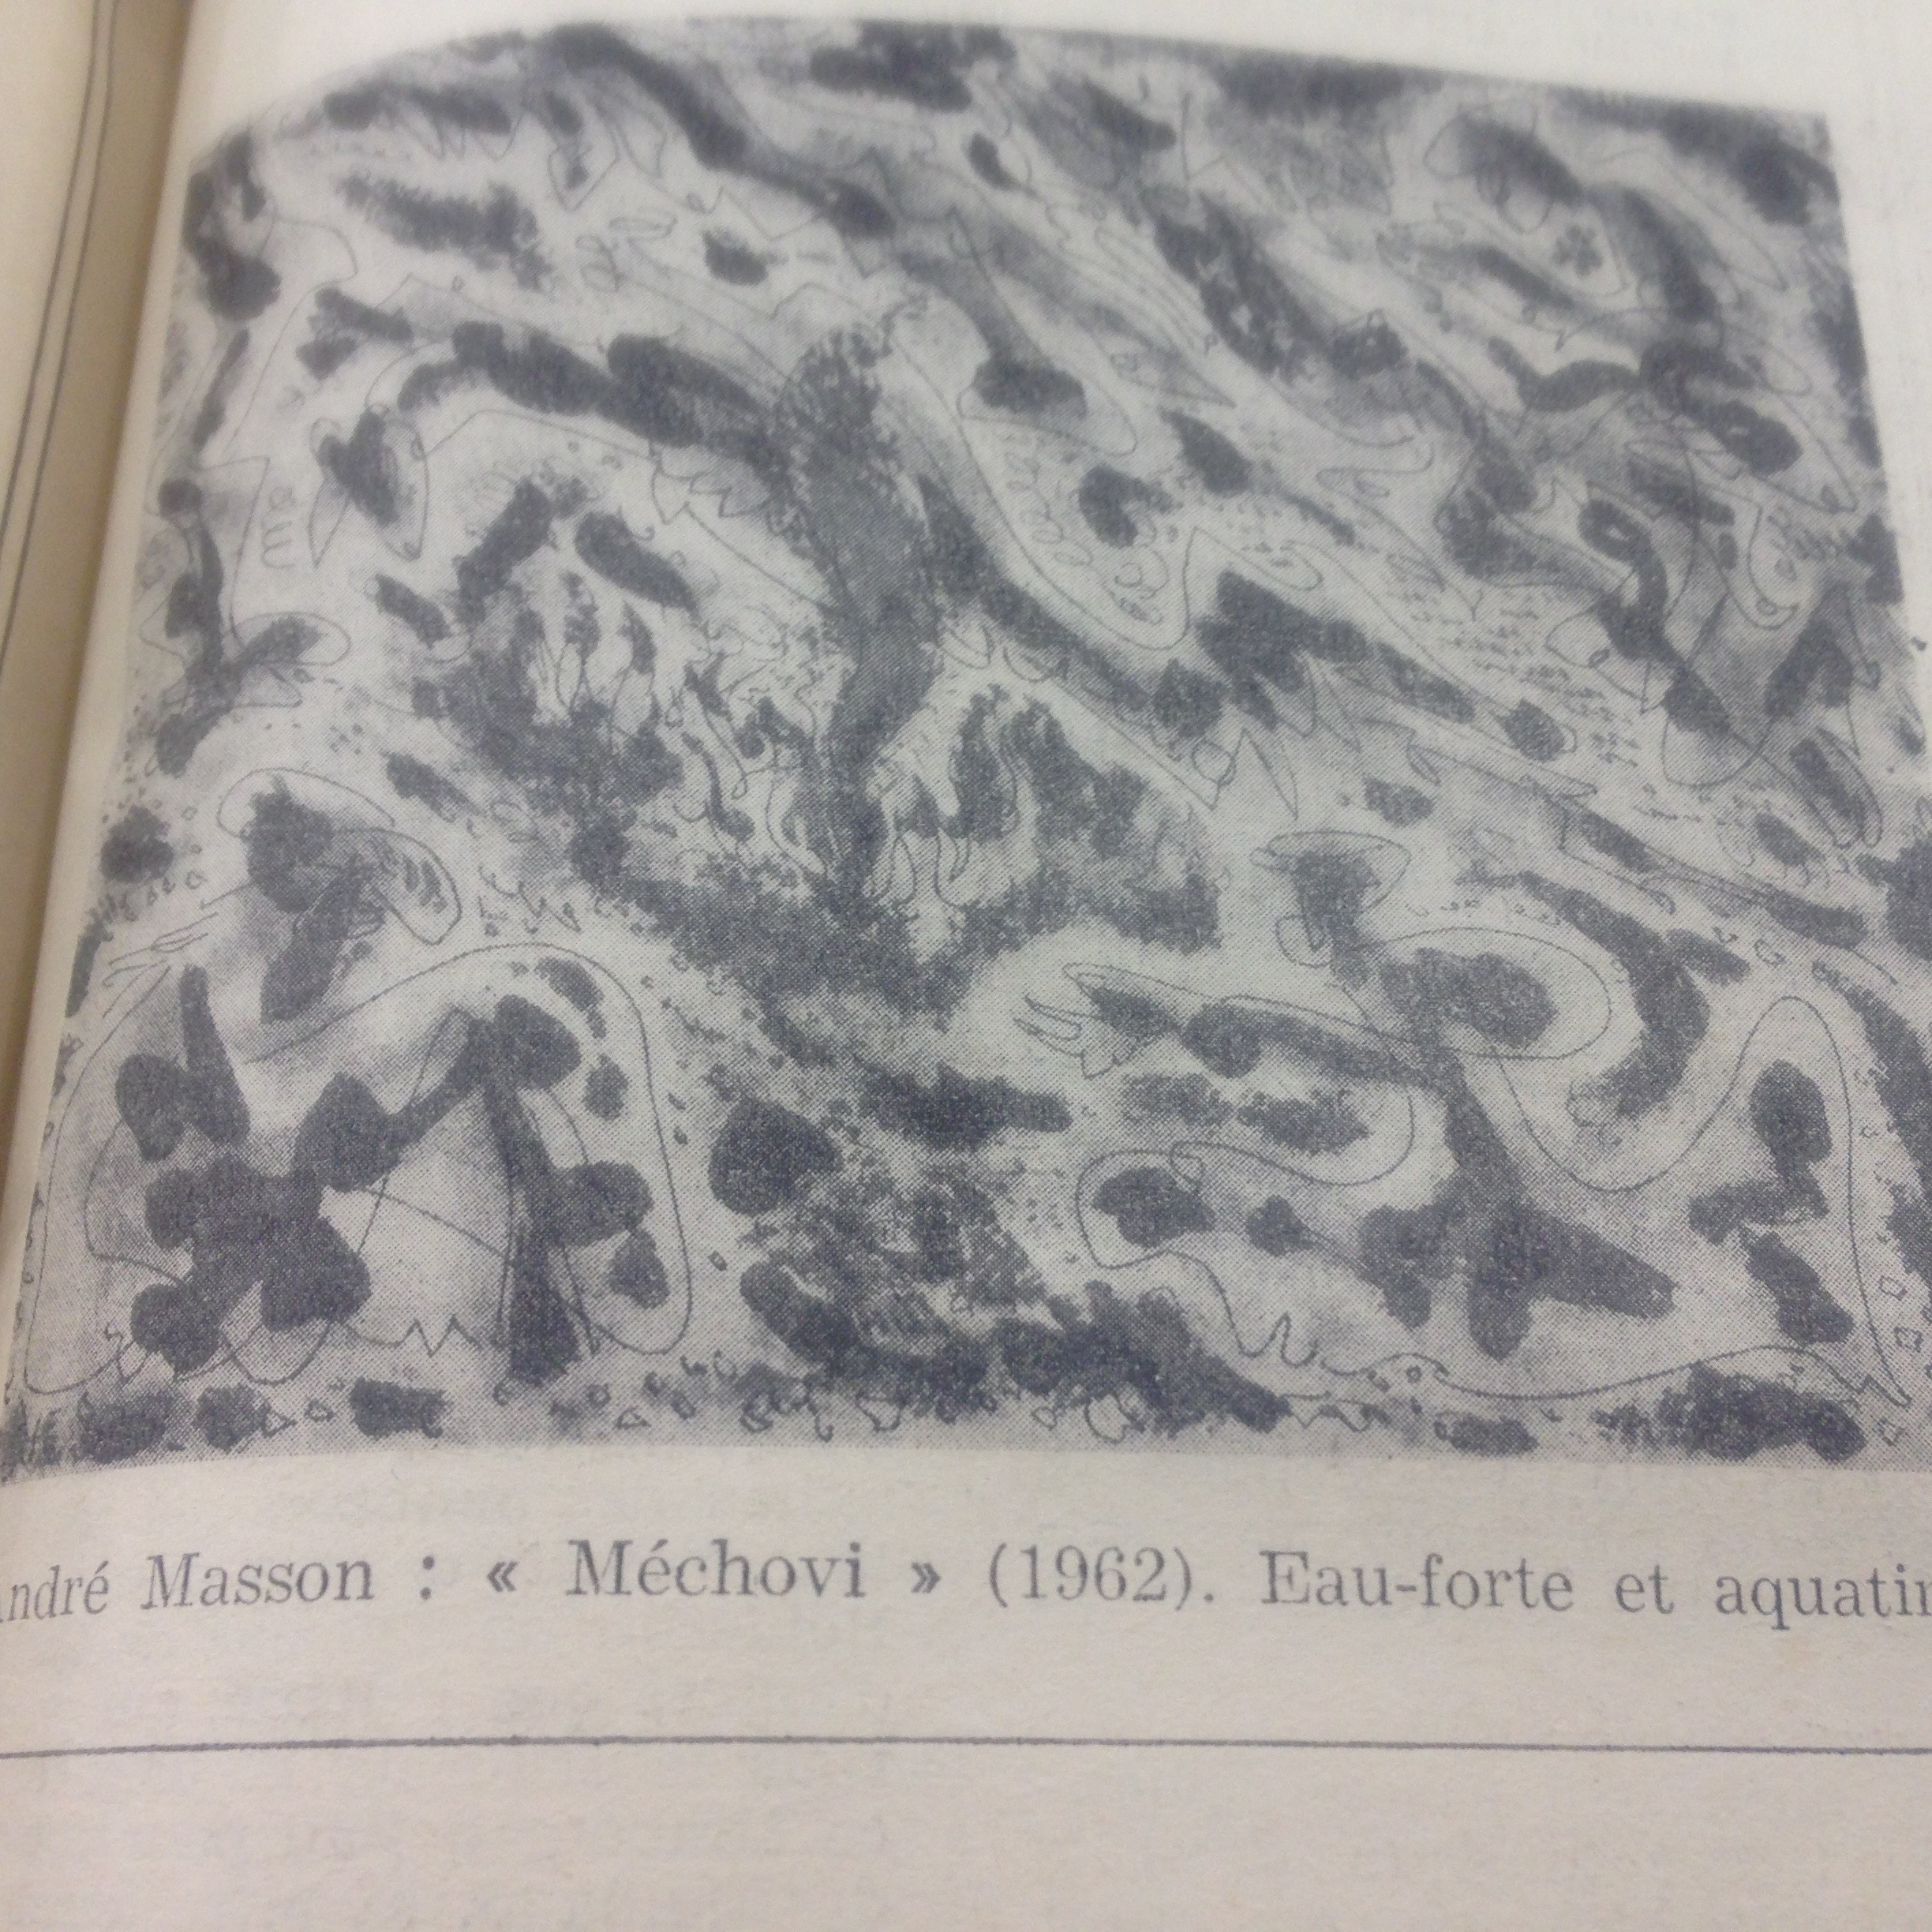
\includegraphics[width=0.75\textwidth]{n1336massonlimbour.jpg}
	\caption{\cite{journallimbour}}\label{fig:limbour}
\end{figure}

	Le choix de l’eau-forte d’André Masson pour illustrer son article opère chez Aragon une référence symbolique à la rencontre avec les vers de Georges Limbour. Dans son article, André Masson traduit la fascination qu’exerçait Limbour sur lui lorqu'il emploie un terme qui pourrait rendre compte de ses propres œuvres : \enquote{Jamais poète ne fut plus indifférent à la gloire et à ses pièges, à tel point qu’il était pour nous une énigme.} L’énigme est une esthétique complète dans l’art d’André Masson, de même que dans l’\oe{}uvre poétique de Limbour. Pour renforcer cette idée, lui-même est associé par Aragon à Rimbaud. Ce qui représente l'hommage suprême pour un ancien surréaliste à propos d’un camarade. En outre, la figure de Limbour justifie d’autant plus cette collaboration qu’Aragon induit lui-même dans son texte rétrospectif des années surréalistes quelle figure médiatrice son ami aura été à la naissance du surréalisme entre le groupe ex-dada de Breton et celui des artistes de la rue Blomet : 

\begin{quote}
On traversait le courant pour aller s’asseoir sur la rive droite où il y avait alors un bout de plage de gravier. Entre temps, Limbour s’était lié à la fois avec la rue Fontaine et la rue Blomet, je veux dire avec les gens qui allaient chez André Breton, et le groupe plus restreint mais plus cohérent des amis d’André Masson. Non que l’on pût alors opposer les uns aux autres, mais les relations y étaient de caractère différent. C’est vers cette époque que, rue Fontaine, on se mit à s’adonner à un sport assez singulier : je veux parler de l’époque dite des \emph{sommeils}.	
\end{quote}


	Néanmoins, malgré cette distinction entre les deux groupes, le grand représentant de cette pratique du sommeil, Robert Desnos, associe André Masson à ce qui semble être la visée de son projet. Lors de son étude commandée par Jacques Doucet en 1927, \emph{Dada Surréalisme}\footcite[p152]{desnos}, dans la dernière partie du tableau de son panorama des deux mouvements jusqu’en 1927, \emph{Le Surréalisme 1924-1927}, \enquote{le rôle d’André Masson} est associé à \enquote{argLa Révolte individuelle}. Une reconnaissance s’établit ainsi entre la grande figure de l’automatique et celle du dessin automatique. Tous les deux aspirant à la liberté au sens le plus large. 

	Ainsi, la \enquote{révolte individuelle} qui pourrait énoncer le projet littéraire du surréalisme tout entier, livre aussi, en même temps qu’un solide point de ralliement pendant cette période vue postérieurement comme un période d’or, le lieu de confrontation de recherches littéraires, et esthétiques, voire même idéologiques, clairement distinctes. 

\section{Polyphonie autour d'un art figuratif dérivé}

\subsection{Les parcours distincts jusqu'à l'expérience surréaliste commune}


Entre le vertige d’Aragon et la fête de Masson se nichent à la fois de profondes idéologiques communes, mais aussi de profondes distinctions. Peut-être en partie parce que ces deux grands surréalistes n’ont pas appréhendé le mouvement avec les mêmes origines : Aragon était avec Breton un fervent dadaïste. Bien qu’André Masson distingue lui-même le style très atypique d’Aragon vis-à-vis de ses amis. Dans son portrait d’Aragon, il qualifie ce dernier de \enquote{romantique}\footcite{desnos}. Pour autant, Masson a aussi raison de relever en mentionnant en 1973 leur rencontre qu’Aragon figure parmi les dadaïstes les plus \enquote{virulents}\footcite[p84]{rebelle}. La convergence qui unit ainsi les deux hommes résiderait donc précisément dans leur polyphonie : tous deux sont hantés par des forces contradictoires. Bien que celles-ci ne se situent pas sur les mêmes axes. Nous avons vu dans sa lettre de 1935 à Georges Batailles quelles réticences a André Masson vis-à-vis du marxisme. 

La première convergence entre eux vient probablement d’Aragon dans \emph{Une vague de rêves}\footcite{vaguedereves}. Il y évoque leur expérience commune de soldats pendant la 1ère Guerre Mondiale. Bien qu’à des postes bien différents comme le sous-entendent les mots d’Aragon pour désigner Masson comme symbole de paix : \enquote{André Masson à tous les carrefours préside aux lâchers des colombes : les beaux couteaux qu’il aura vus partout sont prêts à être enfin saisis.}\footcite[p28]{vaguedereves} Mais la question commune aux deux hommes serait : comment faire image ? Pourquoi Aragon dédie-t-il à André Masson particulièrement \emph{Le Paysan de Paris }? Ce simple geste signifie déjà un écho créatif entre les deux hommes.

En outre, la mythologie est sans doute à la fois une autre source d’inspiration créatrice en même temps qu’elle est traitée différemment chez Aragon et chez Masson.  La mythologie grecque sous la plume d’ Aragon rappelle celle du voyageur à la recherche du vertige. C’est le cas dans sa version du récit du voyage de Télémaque à la recherche de son père Ulysse dans \emph{Les aventures de Télémaque}\footcite{telemaque} à l’époque dada en 1922 jusqu’à \emph{Henri Matisse, roman}\footcite{aragonmatisse}en 1971. On y retrouve la référence courante à la légende du voyage de Pétrarque fasciné par l’île de Thulé qui opère à la fois un jeu de miroir avec celui de Matisse à Tahiti dans les années 30, mais reflète aussi l’exploration intérieure de l’artiste. Dans les deux cas,le mythe est le voyage qui mène au vertige. Chez André Masson, le mythe est indissociable ment lié à la question de la métamorphose. Bien que le topos du voyage chez Aragon corresponde lui aussi à une idée de transformation où le voyage est un lieu d’entre-deux dans le processus de devenir de l’homme. André Masson, lui, traite la métamorphose et la mythologie comme les deux éléments fondateurs de son art : 
\begin{quote}
Comment ne pas écrire METAMORPHOSE avec les grandes lettres alors qu’il est le mot-maître de ma vie et de mon art ? L’esprit de métamorphose et l’invention mythique sont les extrémités du balancier qui m’ont permis de traverser sur la corde raide un monde de tragédie, d’écueils et de souffrances. (Toutefois alternent massacres et bouffonneries. Je suis un pessimiste gai.)\footcite[p8]{memoiremonde}\end{quote}

En conciliant ces deux idées de \enquote{métamorphose} et d’\enquote{invention mythique}, c’est à l’imaginaire qu’André Masson fait référence, autre mot qu’il écrit aussi en majuscules, \enquote{le triomphe de l’IMAGINAIRE dans l’art contemporain.}\footcite[p19]{rebelle}La désignation d’André Masson de l’imaginaire comme apogée de l’art rejoint la définition d’Aragon de l’\oe{}uvre romanesque comme \enquote{aventure de l’esprit}\footcite{sivous}. Le terme est utilisé par Aragon en 1965 dans son article \emph{Si vous m'en croyez}\footcite[p1]{sivous} . Cette désignation à propors de la première \oe{}uvre romanesque de Ristat revient en 1971 à propos du projet des vitraux de Matisse pour la chapelle de Vence dans \emph{Henri Matisse, roman}\footcite[p643]{aragonmatisse}. Elle vaut ainsi pour la création au sens large. Cette idée comporte par nature une part d’imaginaire qui se traduirait par un processus d’évasion de l’esprit. On se rapproche avec cette conception romanesque de l’idée de libération totale, laquelle est l’exigence que se fixe Masson dans ses \oe{}uvres. Quelle que soit le type de liberté, idéologique ou libertaire. 

\subsection{La collaboration, autour du \emph{Con d'Irène}en 1928, et sa réactualisation avec les \emph{ORC}}

Or, cette corrélation de la vision romanesque d’Aragon et picturale de Masson se confond lors du projet \emph{\OE{}uvres romanesques croisées} de 1964 : Célébrés dans \emph{Les Lettres françaises}, le premier tome d’\emph{ORC} est consacré à réédition des \oe{}uvres d’Elsa Triolet et le second à celles d’Aragon, en l’occurence à \emph{Anicet ou le panorama, roman} (1918)  suivi du  \emph{Libertinage }(1924). Or, André Masson désigne ,à plusieurs reprises, dans son texte \emph{Salut [Louis Aragon ]}, Aragon comme \enquote{l’auteur d’Anicet}. Si André Masson connaît et admire Aragon de nom avant leur rencontre, c’est d’abord par goût de son \oe{}uvre Anicet, ce qui fait de l’\oe{}uvre la réelle naissance de l’amitié entre les deux hommes. C’est pourquoi la présence d’\oe{}uvres de Masson parmi celles des artistes qui collaborent à illustrer le tome 2 d’ \emph{ORC} peut apparaître à la fois comme une marque symbolique de leur amitié autour d’une \oe{}uvre qui a nourri les premières discussions entre les deux hommes. Pourtant, ce n’est pas \emph{Anicet} le projet auquel participe Masson, illustré par Picasso, mais au\emph{Libertinage}. Le nom même évoque l’une des plus fameuses collaborations entre les deux hommes : le texte Le Con d’Irène d’Aragon illustré par les fameux dessins érotiques de Masson. Comparer le traitement des dessins sur un thème similaire mais avec autant d’années d’écart pourrait être intéressant. De même qu’une collaboration marquée entre les deux hommes sous le signe du Libertinage. 

Ce signe s’établit en partie dans \emph{Le Con d’Irène}, grâce au croisement esthétique de la description du rêve érotique d’Aragon et des dessins de Masson : dans le rêve comme dans le dessin, l’image livrée est celle d’une ronde de femmes. D’où l’impression de méli-mélo et d’effet d’orgie provoqué par l’entrelacement des corps. C’est la mise en mouvement de l’idée de \emph{Mouvement perpétuel}, d’après le titre du recueil de  1926 , traité au sens libertaire le plus large.


L’évocation des dessins du Con d’Irène, intégré dans le récit fragmenté \emph{Défense de l’Infini}\footcite{defense} de 1928 et brûlées partiellement par leur auteur à l’époque, rappellent immédiatement les dessins automatiques de Masson. Et, pour cause, on peut supposer que le processus de l’automatisme se confond parfaitement avec un tel sujet. D’autant plus que c’est à la même période de l’année 1964 qu’Aragon publie \emph{\OE{}uvres Romanesques croisées}, et particulièrement le tome 2 sur \emph{Anicet ou le panorama, roman} et \emph{Libertinage}. Il commence également à légitimer la \emph{Défense de l’Infini}, c’est-à-dire qu’il revendique en être l’auteur et évoque son histoire personnelle dans ses \oe{}vres. Un croisement s’opère donc entre la collaboration d’André Masson et d’Aragon en 1928 pour \emph{Le Con d’Irène} et celle de 1964 autour de \emph{Libertinage}. Si le  \enquote{Libertinage} peut qualifier le thème du \emph{Con d’Irène}, Aragon exploite le sujet au sens le plus large du terme, avec une insistance qui laisse pressentir sa collaboration avec André Masson, le topos de la liberté : 

\begin{quote}
Ce que je pense, naturellement s’exprime. Le langage de chacun avec chacun varie. Moi par exemple je ne pense pas sans écrire, je veux dire qu’écrire est ma méthode de pensée. Le reste du temps, n’écrivant pas, je n’ai qu’un reflet de pensée, une sorte de grimace de moi-même, comme un souvenir de ce que c’est. D’autres s’en remettent à diverses démarches. C’est ainsi que j’envie beaucoup les érotiques, dont l’érotisme est l’expression. Magnifique langage. Ce n’est pas le mien. Nonobstant ce que je pense du limité de l’expérience, de l’inévitable répétition d’un thème élémentaire et parfaitement réductible à toute autre action indifférente, j’ai le plus profond respect de ceux pour qui cette limitation semble la liberté même. Ils sont les vrais maîtres du monde physique, les parfaits exécuteurs d’une sorte métaphysique de hautes \oe{}uvres, où se résume pour moi spectateur, toute espèce de moralité.\footcite[p266]{defense}	
\end{quote}
 


	Et, en même temps, Aragon dévoile ses limites face à la liberté totale, suggérant une distinction entre l’écrivain qui aspire à cette liberté, et celui qui la possède, l’érotique, en l’occurrence : André Masson. En distinction, l’écrivain se qualifie de \enquote{spectateur} car ne créant pas directement l’érotisme. La collaboration avec André Masson va ainsi  pallier cette limite de l’écrivain : \enquote{J'écrivais donc. Le temps devait être brûlé par quelque pierre infernale. La seule que je connaisse est la pensée, et j’ai dit qu’écrire est ma seule méthode de pensée. J’écrivais. J’ai toujours envié les érotiques, ces gens libres. Ils n’écrivent pas.}\footcite[p270]{defense} La question qui se pose, d’autant plus qu’Aragon ne parle que pour les écrivains, serait : Si les écrivains ne peuvent par nature être libres, en revanche,  les gens libres dessinent-ils ? Toujours est-il qu’avec cette répétition à la fois de l’aspiration de l’écrivain à la liberté et son incapacité à devenir un être libre, André Masson agit non pas comme l’illustrateur des propos d’Aragon, mais comme leur prolongement. Masson n’est pas dans une attitude de reproduction, mais plutôt la continuité de la création de l’érotisme. L'influence du dessin automatique et son traitement particulièrement charnel chez Masson se confond ainsi dans les propos du narrateur. Lors de l'enivrement de son rêve érotique dans une ronde de corps fémininis qui entourent le rêveur :

	\begin{quote}
	Un rêve mit un peu de répit à une surexcitation si continue : six femmes austèrement habillées jusqu’à la ceinture m’avaient entouré pendant que j’étais occupé à nouer les cordes qui retenaient l’échafaudage d’une maison en construction à un anneau où on avait aussi attaché un cheval.
	Elles avaient fait une ronde autour de moi, courbées, se passant l’une l’autre le bras autour de la taille pour aller de la main gauche tripoter le bouton de leur voisine, tandis que leurs langues farfouillaient à droite les culs de celles qui les tortillaient pour les toucher. Dans mon rêve, c’était tout naturel, et ça tournait. Et les filles me frôlaient de leur vulve gonflée.\footcite[p260]{defense}	
	\end{quote} 
	
	\begin{figure}[H]
        \centering
        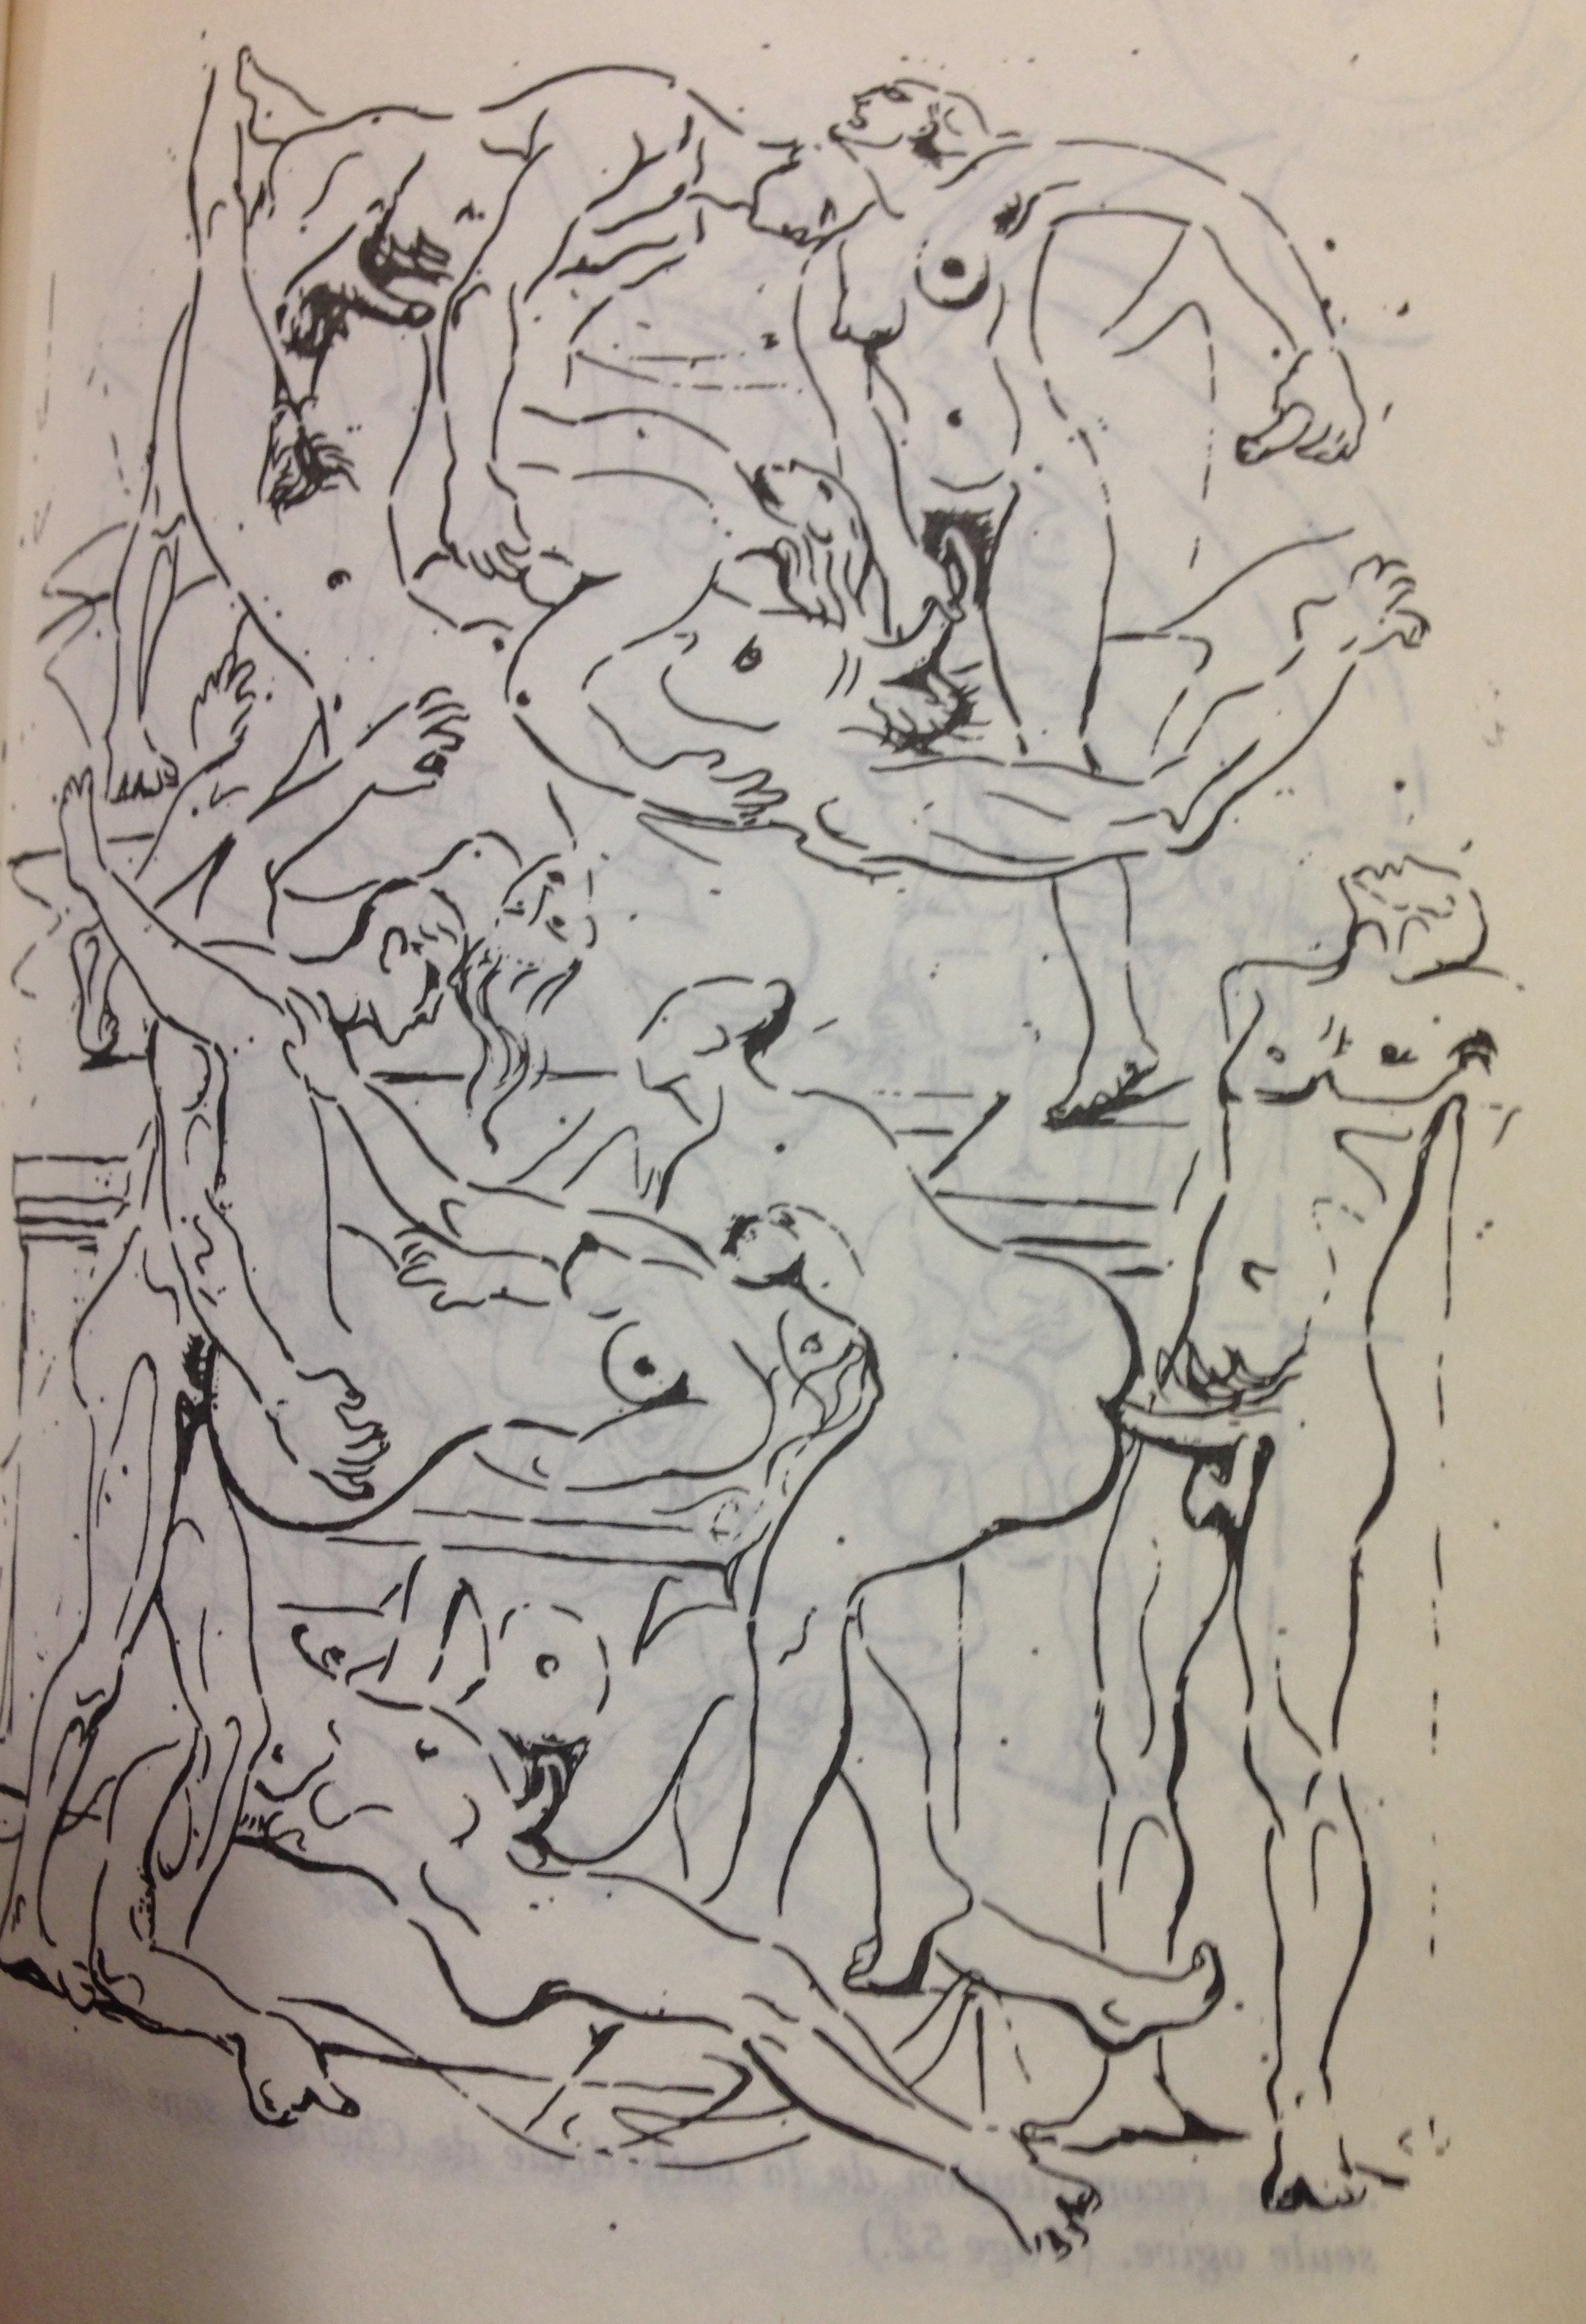
\includegraphics[width=0.75\textwidth]{I13}   
        \caption{\emph{Le con d'Irène}}\label{fig:irene1}
	\end{figure}

	 L'érotisme est ainsi crée par le mouvement propre à la forme de la ronde, où, tout comme Masson le revendique dans le dessin automatique en général, de l'onirisme naît l'organique. La création du libertinage sous la forme du mouvement érotique est ainsi une création partagée. Elle naît ainsi du rêve du narrateur pour exister par les traits du dessinateur. 

On peut souligner que ce thème du libertinage ira dans l'imaginaire Aragon jusqu'à immerger dans celui de Masson, comme le manifeste la nouvelle \emph{Min mini mi,} inscrite dans le recueil du \emph{Mentir-Vrai} :

	 \begin{quote}
	 Ce que je me proposais au début de cette phrase de définir, c’était, ou plus précisément, c’est la limite entre le pouvoir de dire et le pouvoir d’interdire, par l’invention purement abstraite du concept d’obscénités pour abréger les choses et sortir du labyrinthe où nous nous croyons enfermés en tête à tête acec ce qui est la forme moderne du Minotaure.\footcite[p494]{mentirvrai}\end{quote}

	 Comment ne pas non seulement immédiatement reconnaître l'imaginaire d'André Masson ? On y décerne par conséquent l'hommage d'Aragon pour un ami et artiste qui représente pour lui un maître de l'érotisme. Leur collaboration passée avec \emph{Le Con d'Irène} encourage l'idée que l'usage de la métaphore du labyrithne et du Minotaure dans son propos sur l'érotisme, Aragon constitute indéniablement une référence à Masson. Ce qui siginfierait que ces lignes sur l'érotisme sont aussi des mots d'amitié à l'égard d'André Masson comme le reflète l'emprunt à l'imaginaire proprememt massonien. Si l'on prend en compte que la nouvelle date de 1970, la période correspond à la période d'hommage d'une amitié discrète au milieu de toutes les autres durant la période surréaliste et que les deux hommages à présent âgés et derniers sruvivants de cette génération remettent au goût du jour. On se situe ainsi dans la même logique que la \emph{Cantate à André Masson}, de 1977. L'hommage est peut-être même plus intense grâce à ce procédé lyrique, puisque l'imaginaire de Masson se substitue à son propre nom.
	 
	 D'autant plus que cette référence massonienne déborde la partie surréalsite : la revue \emph{Minotaure}de Bataille et de Masson date de 1936, c'est-à-dire à une période où Aragon et Masson poursuivent des chemins distincts. Tout en correspondant pour les deux hommes à une période journalistique riche: \emph{Commune} et \emph{L'Humanité} pour Aragon, la revue \emph{Minotaure} pour Masson. Cette période des années 1930 correspond aussi à celle où Masson peint et dessine une série d'\oe{}uvres, \emph{Tauromachie} où l'image du taurau qui le hante est non seulement associé au symbole de la corrida dans cette période de la guerre civile en Espagne dans laquelle il vit. Mais la corrida est aussi un moment du corps du taureau pris en mouvement, ce que Masson met en scène dans une lutte de couches de corps différents. Mais le \emph{Minotaure} de Masson va s'associer dans son imaginaire à d'autres figures mythologiques. En particulier, avec celle de Dionysos, et cette idée de profusion qui caractérise ses \oe{}uvres, ce qu'Aragon qualifie d'\enquote{illimité} dans cette nouvelle sur l'érotisme. Autrement dit, Aragon reprend le terme dont Masson s'inspire pour décrire son esthétique. L'érotisme est profusion par nature, de même que la \enquote{fête} selon Masson. Elle est pour le peintre la notion antithétique à l'asservissement. L'érotisme est une forme de liberté par cette profusion. Toujours est-il que, dans sa nouvelle \emph{Min mini mi},lorsqu'il fait l'éloge du lyrisme, Aragon pourrait tout aussi bien décrire un tableau de Masson : 

\begin{quote}
Je voudrais dire qu'à mon sens il n'y a d'érotisme...que l'érotisme vrai, dans sa nature grandiose, ne commence qu'au-delà de l'imitation qu'il ne mérite son nom magnifique qu'à partir du moment où il dépasse ce qui est déjà, pour ouvrir à l'imagination des domaines qui ne sauraient connaître de limites, introduire dans les esprits le sens de l'illimité, jusqu'à donner le vertige de l'impossible.\footcite[p496]{mentirvrai}\end{quote}

L'idée de l'érotisme chez Aragon est par essence lyrique. De même que dans \emph{Le Con d'Irène}, l'écriture tend à devenir lyrique tout en signifant ses propres limites : elle n'a pas la capacité d'accéder à l'érotimse. Aragon avait-il en tête des \oe{}uvres de Masson en écrivant ces lignes ? Il n'empêche que l'éloge de l'érotisme sur lequel s'achève la nouvelle est encouragé par l'imaginaire mythologique de Masson. Le même épisode du labyritnhe et la figure du Minotaure véhiculent l'érotisme. Repousser les limites, comme l'offre l'érotisme, passe aussi par la possbilité de l'hybridité. Dans l'érotisme, l'hybridité passerait par l'entremêlement des corps. Ce que Masson représente dans \emph{Le Con d'Irène} par l'intermédiaire du dessin automatique. Mais aussi avec l'exemple du Minotaure avec l'homme sans tête au même nom que la revue qu'il illustre, \emph{Acéphale}. Sans compter que cette recherche de \enquote{l'illimité}, présente dans les mots d'Argon ici sous le signe du \enquote{vertige}, et chez Masson sous celui de \enquote{fête}, idée qu'il reprend à Delacroix, renforce l'idée que la recherche de l'érotisme s'approche de la liberté totale du créateur. Aragon décrit tout autant l'esthétique de Masson. Peut-être l'érotisme agit-il alors sur les deux hommes comme une entreprise philosophique. Elle illustre une forme utopique et uchronique à laquelle ils aspirent, commencée en 1926 et toujours à l'honneur en 1970. 


\begin{figure}[H]
   \centering
   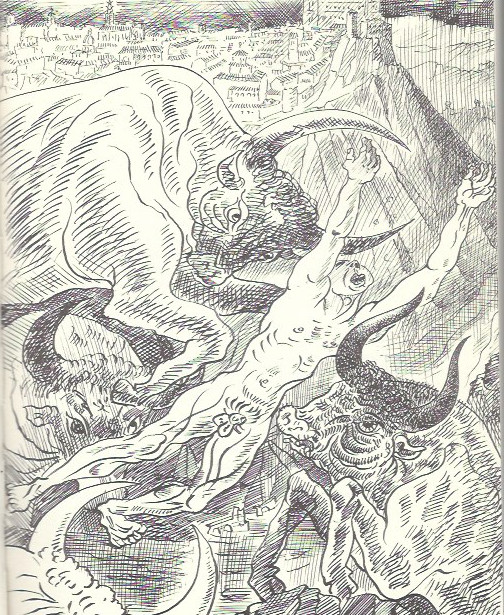
\includegraphics[width=0.75\textwidth]{Tauromachie1935.jpeg}
	\caption{\cite{noel}}\label{fig:Tauromachie1935}
\end{figure}

\begin{figure}[H]
   \centering
   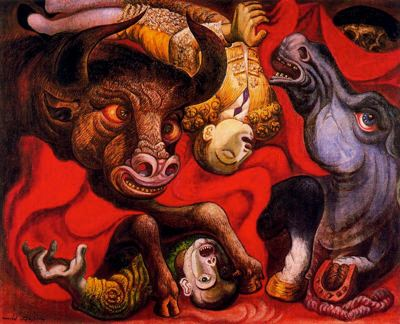
\includegraphics[width=0.75\textwidth]{Tauromaquia1937.jpg}
	\caption{}\label{fig:Tauromachie1937}
\end{figure}


	Ainsi, une telle collaboration axée sur un axe aussi spécifique n’est pas anodin : Elle témoigne d’une même recherche esthétique chez Aragon et Masson. 
% rajouter des oeuvres de Masson sur le Minotaure.
\subsection{Le théâtre comme geste d'amitié entre les deux hommes}

	Dans \emph{Les Lettres françaises}, la présence d’André Masson est celle d’un fidèle le discret. Elle est celle du lecteur des premières du journal. Et c’est sous la direction d’Aragon, particulièrement dans les années 60, qu’André Masson intervient le plus souvent ou que sa production artistique est le plus recensée. Auparavant, dans les années 50, les réserves d’André Masson sur le stalinisme le rendent plus discret. D’autant plus que lui-même est fortement marqué par sa période d’exil aux Etats-Unis, immensément riche pour lui en productions, expositions, conférences et découvertes. Il le revendique une fois rentré en France : \enquote{C’est en Amérique que pour moi les choses se sont concentrées, là où je suis allé le plus loin, où j’ai mûri.} Un numéro des \emph{Lettres françaises} de 1957 recense en pleine Guerre Froide le tournant artistique de Masson. Il quitte la perspective bestiale de l’homme vers une autre plus pacifique. Comme il vient seulement de s’installer définitivement en Provence, on imagine combien cette évolution s’est construite en grande partie lors de son exil américain. Néanmoins, l’\oe{}uvre romanesque d’Aragon est elle aussi en pleine évolution au moment où André Masson, après un passage près de Poitiers, s’installe directement en Provence après son exil. Une transition créatrice s’établit donc pour les deux hommes, au même moment.\emph{Les Lettres françaises} apparaît ainsi comme le lieu de visibilité des transitions respectives des deux hommes. Ce qui donne lieu à des croisements qui ne font que se renforcer : il révèle entre 1964 et 1965 une même attirance particulière pour le théâtre. Plus particulièrement, la place de l’art pictural dans le théâtre. Si Aragon consacre en novembre 1965 un numéro sur le plafond de l’Odéon peint par André Masson, il s’enthousiasme déjà dès l’automne 64 pour le plafond de Chagall de l’Opéra Garnier. Aragon et Masson se rencontrent donc à la même période pour une même fascination pour la forme circulaire des plafonds d’une salle de spectacle.Seulement, cette attirance partagée pour le théâtre dans le courant des années 64-65 correspond à un phénomène équivalent aux \emph{ORC} qui reviennent rétrospectivement sur d'anciennes collaborations : La toute première expérience de Masson familier du monde du théâtre, est née à l'origine pour une pièce d'Aragon qui n'a pas pu voir le jour, mais dont Masson avait déjà réalisé des maquettes : 
\begin{quote}
Quand je dis mes débuts au théâtre datant des \enquote{Présages}, je fais erreur. Louis Aragon vers 1924-1925 me demanda de faire la décoration de sa pièce \enquote{L'armoire à glace un beau soir} qui devrait se jouer au Théâtre des Bouffes du Nord. Je fis la toile du rideau et me préparais au reste quand une brouille du poète avec le directeur interrompit ce bel effort. Seule la maquette du rideau était toujours restée au-dessus de son lit.\footcite[p19]{catalogue}
\end{quote}
	
	 Que cette pièce d'Aragon n'ait pas pu aboutir n'enlève rien à la manifestation d'un désir de collaboration artstique entre les deux hommes. Elle advient dès le moment de leur recontre. Lorsque les artistes de la rue Blomet correspondent de plus en plus vers la rue Fontaine chez Breton, et deviennent membres du groupe surréaliste. Par ailleurs, comme au temps du surréalisme, cette passion artistique est liée aux histoires d’amitiés : Aragon et Masson sont tous les deux très liés au directeur de l’Odéon, le comédien et metteur-en-scène Jean-Louis Barrault. On pourrait même attribuer à la figure d'Aragon ce que Jean-Louis Barrault déclare pour lui-même et Masson dans son texte pour l'exposition \emph{André Masson et le théâtre}, \enquote{Avec André Masson, nous n'avons jamais cessé de nous répondre, avant même de nous interroger.}\footcite[p90]{catalogue}


	 Ainsi, un phénomène de polyphonie et de convergence apparaît devant ces collaborations des jeunes âgées des deux hommes dont ils font témoignange et prolongement à la lumière de leur mémoire d'hommes âgés devant leurs jeunes années. Un second temps à la fois d'amitié et de création naît dans le courant des années 60 entre Aragon et Masson, à la fois pour confondre leurs souvenirs surréalistes, et plus encore pour les prolonger en adapatation avec les nouveaux enjeux esthétiques qui les imprègent. \emph{Les Lettres françaises} deviennent sous la direction d'Aragon ce lieu d'existence du témoigange et de correspondances entre les deux hommes dont on peut se demander si la revue \emph{Les Lettres françaises} n'a pas été à la fois un lieu d'échange mais aussi l'un des prétextes à cet échange devant leur attachement commun à la revue. 

 